\documentclass[12pt,a4paper]{article}
\usepackage[utf8]{inputenc}
\usepackage[english]{babel}
\usepackage{amsmath}
\usepackage{amsfonts}
\usepackage{amssymb}
\usepackage{graphicx}
\usepackage{parcolumns}
\usepackage[left=2.cm,right=2.cm,top=2.cm,bottom=2.cm]{geometry}
\usepackage[final]{pdfpages} %serve per aggiungere altre pagine pdf al file

\author{Davide Bazzanella}
\title{Improving phase-matching of FWM with temperature}

\begin{document}
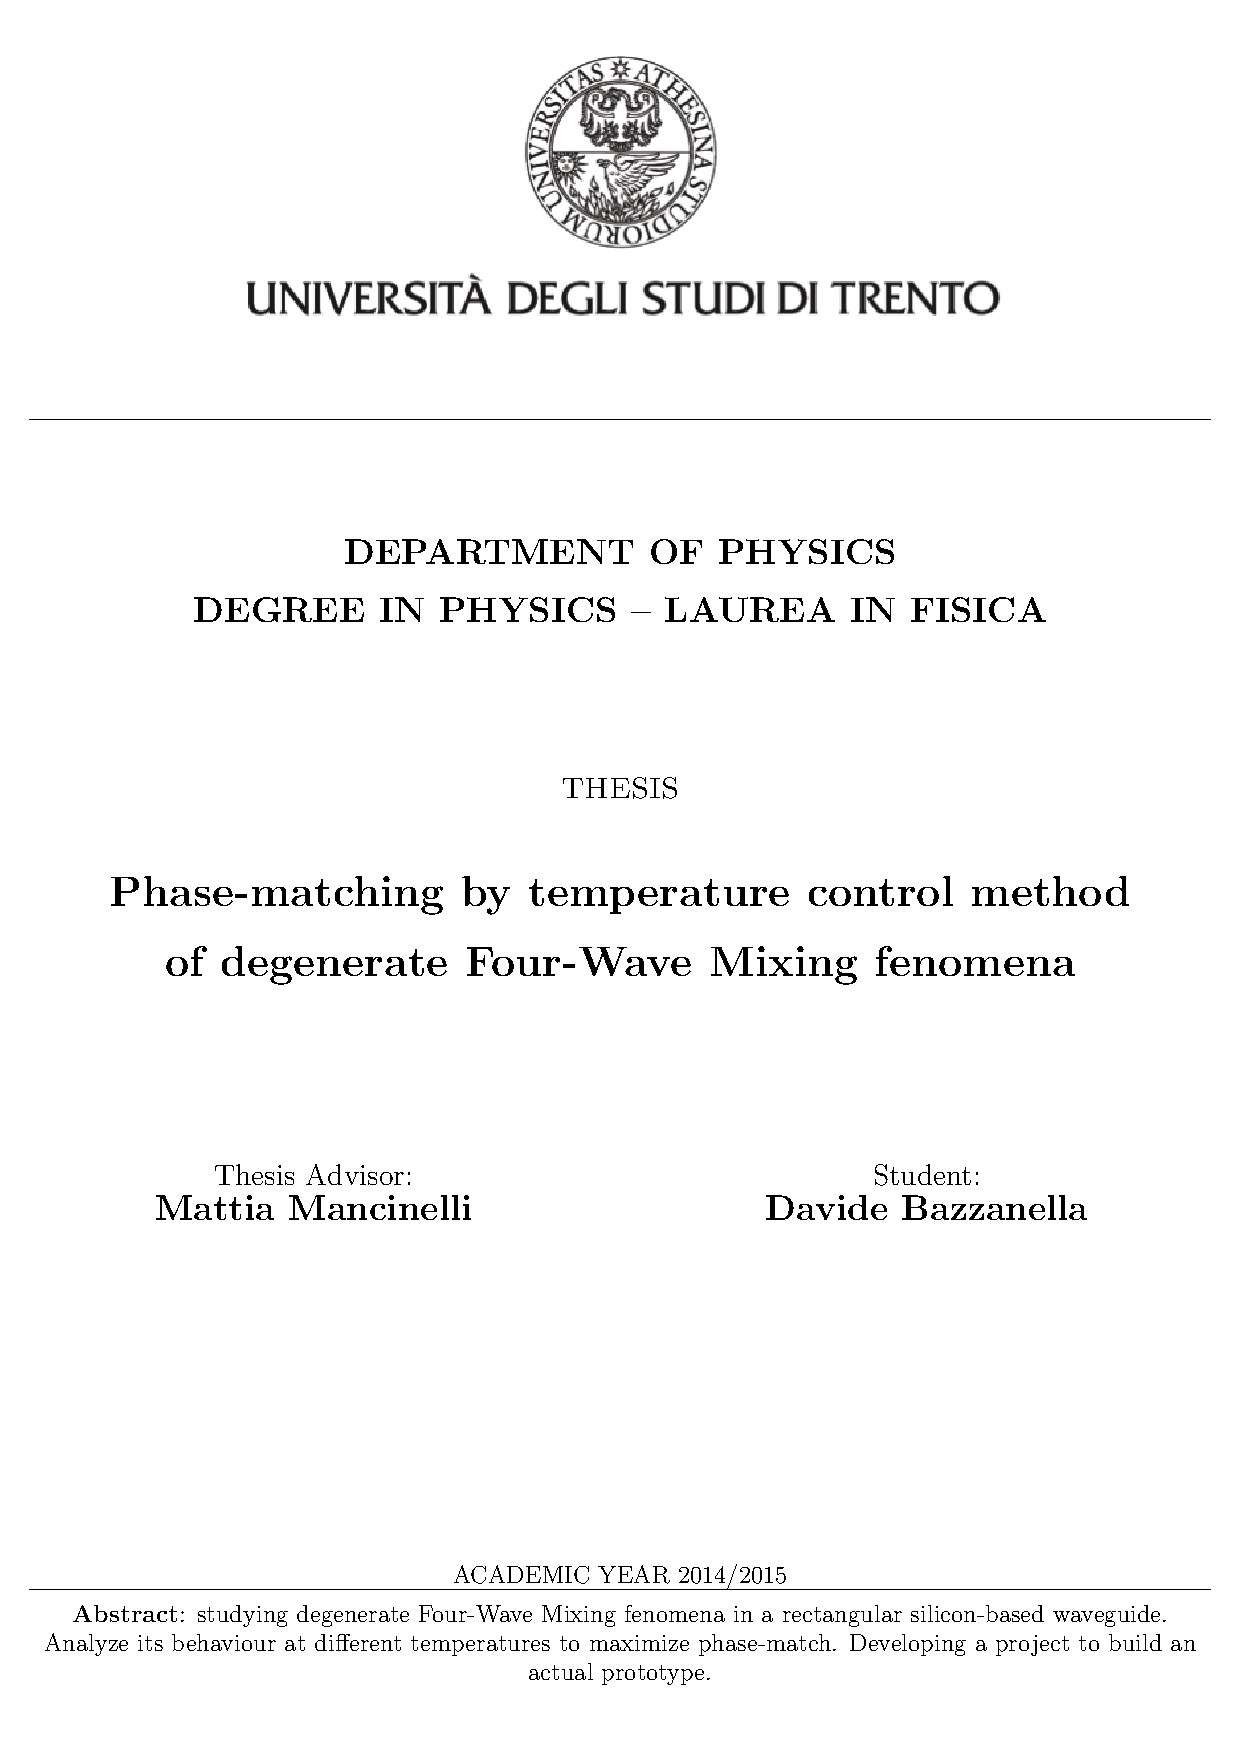
\includepdf[pages={1}]{intestazione.pdf} % \documentclass[11pt,a4paper]{article}
\usepackage[utf8]{inputenc}
\usepackage[english]{babel}
\usepackage{amsmath}
\usepackage{amsfonts}
\usepackage{amssymb}
\usepackage{graphicx}
\usepackage{parcolumns}
\usepackage[left=0.5cm,right=.5cm,top=.5cm,bottom=.5cm]{geometry}

\begin{document}

\begin{titlepage}
\begin{center}


\includegraphics[width=0.7\textwidth]{unitn_logo.png}~\\[1.2cm]

\hrule
$$$$
$$$$

\textsc{\LARGE \textbf{DEPARTMENT OF PHYSICS}}\\[0.5cm]
\textsc{\LARGE \textbf{DEGREE IN PHYSICS – LAUREA IN FISICA}}\\[2.5cm]
\textsc{\Large THESIS}\\[1.3cm]

{ \huge \bfseries Phase-matching by temperature control method}\\
[0.5cm]
{ \huge \bfseries of degenerate Four-Wave Mixing fenomena}\\
[3.0cm]

% ATTENZIONE! Ha bisogno del pacchetto parcolumns per funzionare
\begin{parcolumns}{2}
   \colchunk{\Large Thesis Advisor:\\ \LARGE \textbf{Mattia Mancinelli}}
   \colchunk[2]{\Large Student:\\ \LARGE \textbf{Davide Bazzanella}}
\end{parcolumns}
$$$$
$$$$
$$$$
$$$$
$$$$
$$$$
$$$$
$$$$

\large ACADEMIC YEAR 2014/2015
\hrule
\vfill
\textbf{Abstract}: studying degenerate Four-Wave Mixing fenomena in a rectangular silicon-based waveguide. Analyze its behaviour at different temperatures to maximize phase-match. Developing a project to build an actual prototype.

\vfill

{\large}

\end{center}
\end{titlepage}

\end{document}

\newpage
\section{Introduction}
\subsection{Motivation}
\subsection{Four-Wave Mixing}
Four-Wave Mixing (FWM) is a nonlinear optical effect

\section{Linear optics}
In linear optics the technology for trasmitting a light wave by confining it in a finite space is the guided-wave optics.
The instruments employed for achieving such purpose are called waveguides.
\subsection{Silicon waveguides}
Silicon waveguides are dielectric waveguides and make use of the interface between two media with different refractive index.
Precisely they exploit the phenomenon of total internal reflection, which states that if a propagating wave reaches a boundary between two mediums, one with higher refractive index ($n_H$) and another with lower refractive index ($n_L$), with an angle of incidence (relative to the norm of the interface) greater than the \textit{critical angle}, then the wave is completely reflected in the first medium.
%accorciare la precedente frase%
The critical angle can be obtained by the Snell law.

$$	\theta_C = \arcsin \left( \frac{n_L}{n_H} \right)$$

Silicon waveguides are composed by core and cladding \textbf{(?)}. %is called cladding only for fiber or also for slab/strip wg?
The former is the higher refractive index medium in which the wave is confined, the latter is the lower refractive index medium which surrounds the core, thus creating the interface. Theoretically the cladding could also be vacuum.

Considering an ideal dielectric waveguide (no absorption) and the total field distribution as sum of transverse electromagnetic (TEM) plane waves is possible to study the propagation of the wave along the waveguide with an electromagnetic analysis.
Furthermore it can be shown that not all field distribution are transmitted through the waveguide without energy loss.

% Modes are fields that maintain the same transverse distribution and polarization at all locations along the waveguide axis.
Those field distributions, which maintain the same transverse distribution and polarization at all locations along the waveguide axis, are called \textbf{modes}.
These modes can be categorized in two main groups, depending on the polarization of the wave: transverse electric (TE) modes and transverse magnetic (TM) modes, which have respectively the electric and magnetic field transverse to the waveguide axis.
Both TE and TM modes can be again classified by their order, that is proportional to the number of maxima of the modulus of the electric and magnetic fields in the core section.


\subsection{Rectangular dielectric waveguides}
In a rectangular dielectric waveguide the classification of modes need two indexes because we have two degrees of freedom.

\section{Non-linear optics}

\subsection{Third order effect: Four-Wave Mixing}

\section{Simulating and coding ?}

\section{Prototyping}
\subsection{Heater configurations}
\subsection{Different geometries}

\end{document}